\subsection{Getting on to the System}
\begin{itemize}
	\item{Sign up your account}
	\newline
	You will need to add an account in order to be able to sign in on the system.
	\begin{figure}[H]
	    	\centering
	    	\fbox{\includegraphics[width=0.5\textwidth]{SignUP}}
	    	\caption{Sign Up}
	    	\label{fig:Learning rate 0.1}
   	\end{figure}
	\item{Sign in}
	\newline
	After your account has been created, you will be able to sign in.
	\begin{figure}[H]
	    	\centering
	    	\fbox{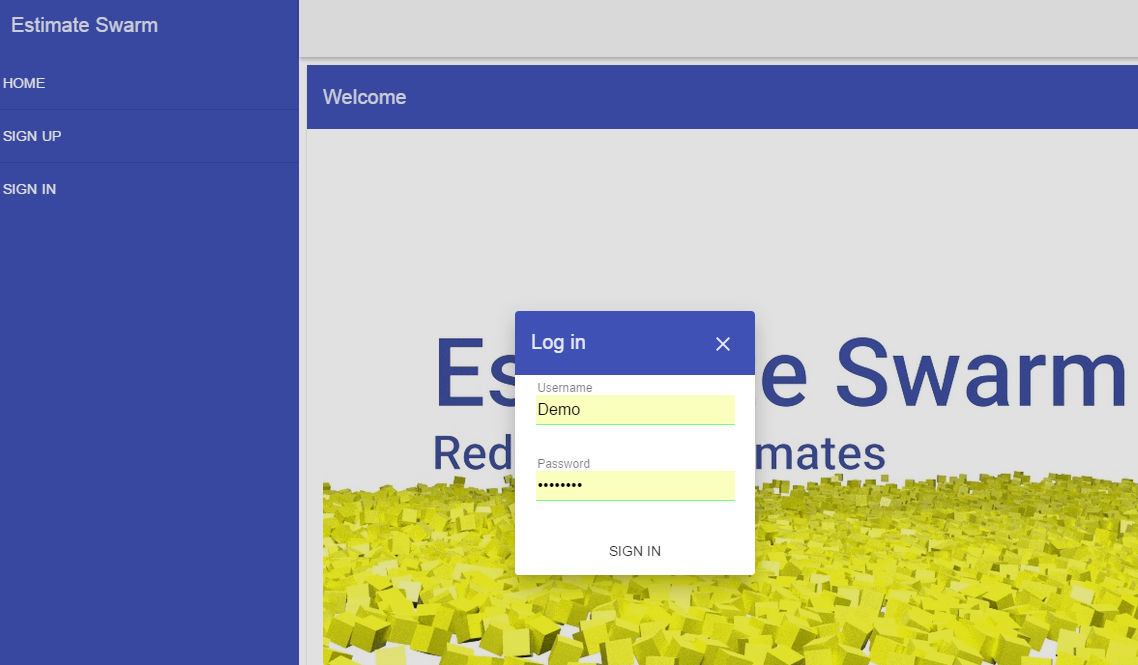
\includegraphics[width=0.5\textwidth]{login}}
	    	\caption{Login}
	    	\label{fig:Learning rate 0.1}
   	\end{figure}
\end{itemize}
\subsection{My Profile}
\begin{itemize}
	\item{Edit Profile Details}
	\newline
	After you account has been created and you are signed in, you can access your information on the "Profile" page. You can navigate there from any other page, while signed in, by clicking on the "Profile" tab on the left hand side navigation. Here you can edit your account information as shown in the figure below. After you are done editing, you can save your changes by clicking the "Save Profile" button at the bottom of the screen.
	\begin{figure}[H]
	    	\centering
	    	\fbox{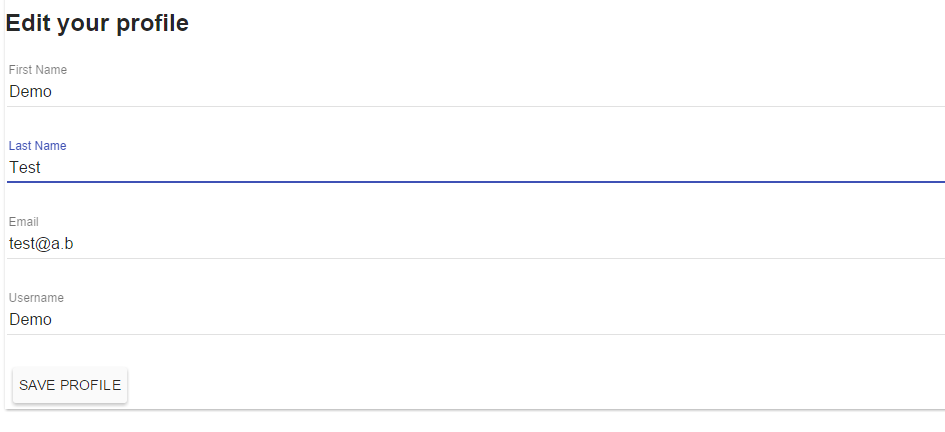
\includegraphics[width=0.5\textwidth]{profile}}
	    	\caption{Profile Page}
	    	\label{fig:Learning rate 0.1}
   	\end{figure}
\end{itemize}